%\section{The As-Is Architecture}
\section{As-Is}
\label{sec:as_is}
The As-Is architecture of J.D.H. Insurance is derived based on their most important processes. From these processes the information systems, information objects and technical infrastructure can be identified. The following sections will present each of these important processes and analyze the architecture on different attributes in the MAP metamodel. The full As-Is architecture can be viewed in Appendix A, divided into 4 views; the Business layer, Application layer, Infrastructure layer and the information layer. The attached iEaat file JDHInsuranceAsIs also contains the full As-Is model.
%
\subsection{J.D.H. Insurance’s most core processes}
\label{sec:coreShit}
The models presented in this section considers the As-Is state of the enterprise architecture. The following subsections will describe the important functions in J.D.H. Insurance and each function will be followed by a model explaining the business layer of the process.
%
\subsubsection{The Ordering of an Insurance}
\label{sec:order}
To order an insurance the customer is able to browse J.D.H. Insurance’s website for the insurance they would like to apply for. The customer is then able to download a paper application form and send it to J.D.H. Insurance by mail for the company’s order managers to register the order and to send an order status response back to the customer before the order of an insurance is completed. Figure 1 shows the business services available for the customer and what processes they are realised by.
\begin{center}
	\begin{figure}[H]
		\centering
		\setlength\fboxsep{7pt}
		\setlength\fboxrule{0.5pt}
		\fbox{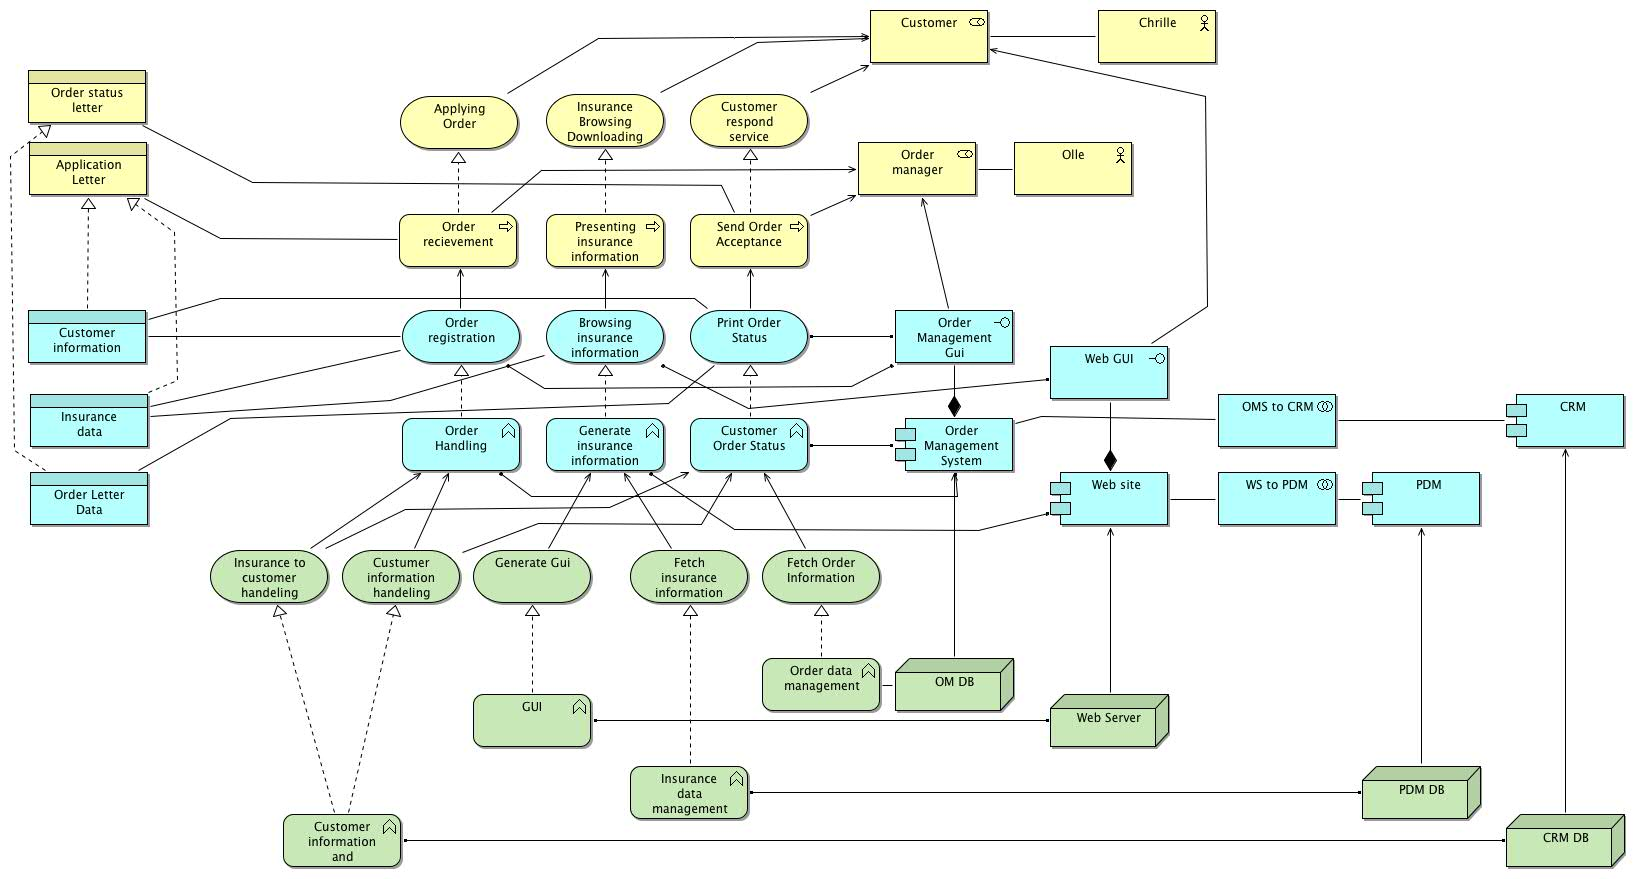
\includegraphics[scale = 0.252]{images/order.jpg}}
		\caption{Ordering an insurance (\emph{ArchiMate})}
		\label{fig:archi_order}
	\end{figure}
\end{center}
\subsubsection{The Process of Claim Registration}
\label{sec:claim}
To claim compensation, the customer are able to download a paper claim application from the website. The application, including customer information and claim description, is sent to J.D.H Insurance by mail which is received by a claim administrator which registers it in the Claim management system by hand. A Claim Evaluator evaluates the claim application and compensates the customer in case of valid claim. Either way the claim evaluator notifies the customer by sending a letter with his answer to the claim. Figure 2 displays the services available to the customer and the underlying process. It also shows the processes which the evaluator and administrator executes.
\begin{center}
	\begin{figure}[H]
		\centering
		\setlength\fboxsep{7pt}
		\setlength\fboxrule{0.5pt}
		\fbox{\includegraphics[scale = 0.245]{images/claim.png}}
		\caption{Claim registration (\emph{ArchiMate})}
		\label{fig:archi_claim}
	\end{figure}
\end{center}
%
\subsubsection{Support Processes}
\label{sec:support_processes}
J.D.H. Insurance provides various support services for their customers and possible customers, which includes support by phone or e-mail. Each support service are described in the following subsections.
\paragraph{Phone Support}
\label{sec:phone}
The customer has the option to call in to J.D.H. Insurance for support. The process works like following: the customer makes a call, whereupon this call gets registered by the phone support system and then placed in a stack by the phone dispatcher. The call then gets handled by someone in the support team which will try to solve the problem over the phone. While trying to solve the problem at hand, the supporter is provided with a FAQ service that will help in the problem solving. The results of the solving process is directly reported back to the customer in the call.
\begin{center}
	\begin{figure}[H]
		\centering
		\setlength\fboxsep{7pt}
		\setlength\fboxrule{0.5pt}
		\fbox{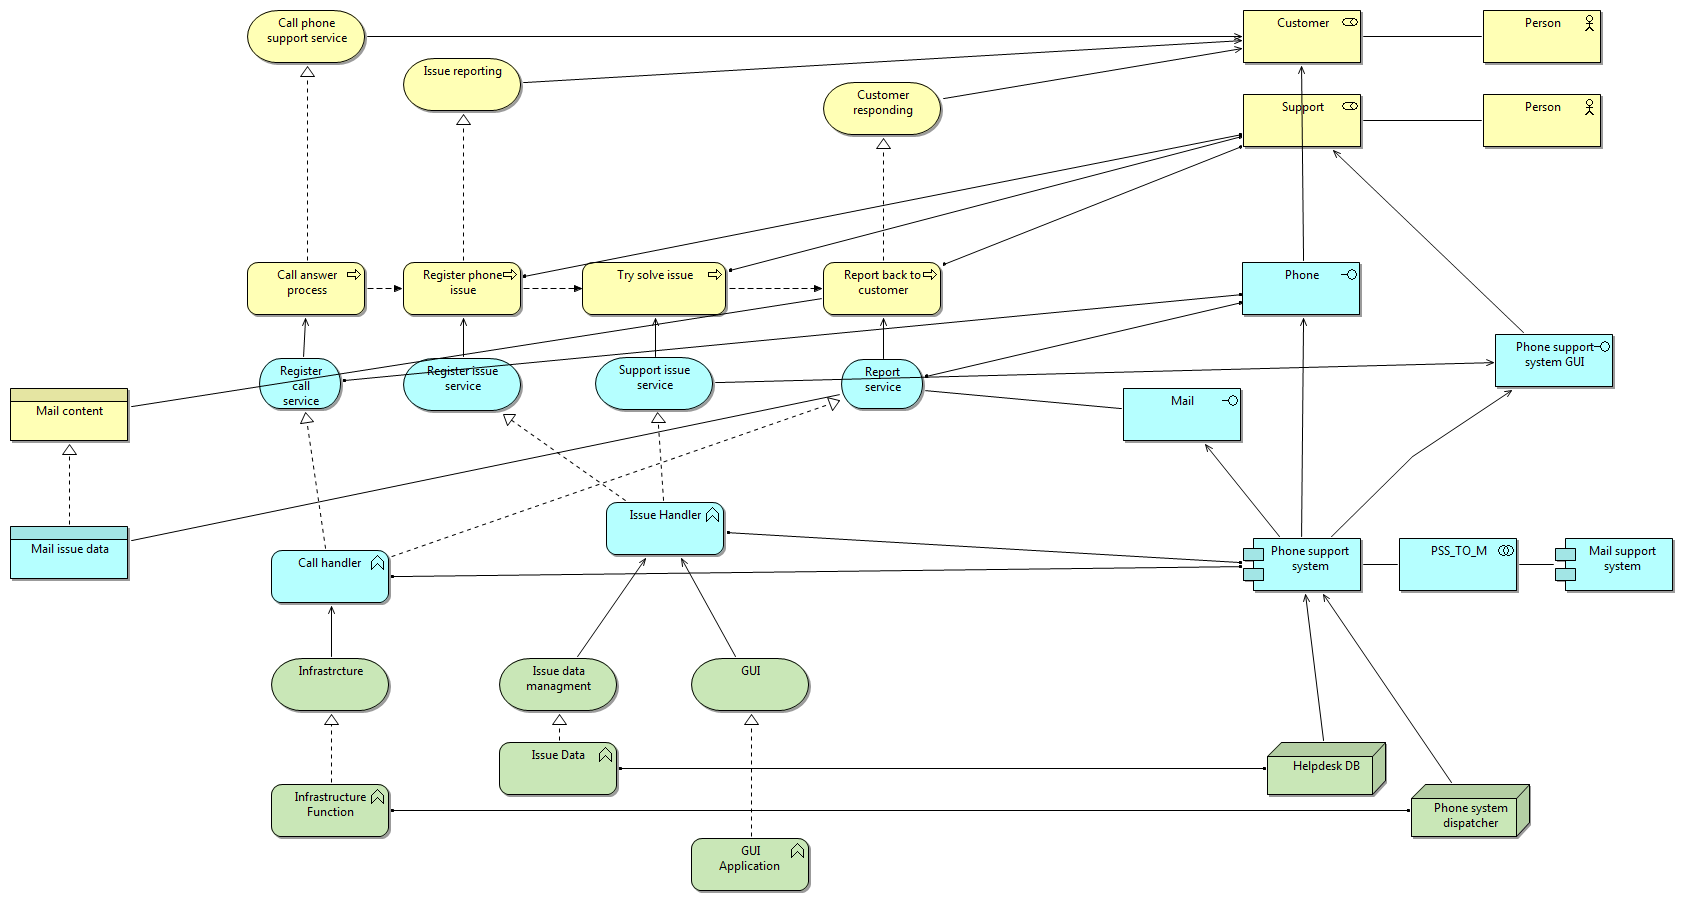
\includegraphics[scale = 0.25]{images/phone.png}}
		\caption{Customer support via telephone (\emph{ArchiMate})}
		\label{fig:archi_phone}
	\end{figure}
\end{center}
%
\paragraph{E-Mail Support}
\label{sec:mail_support}
The customer is able to send an e-mail to get support from J.D.H. Insurance’s support team. The e-mail sent to the support team gets registered in the mail support system for help desk team to try solve. When the issue is handled the employee handling the issue sends an e-mail back to the customer including the results from the investigation. Figure 5 shows the services available to the customer and what processes the support team executes to enable e-mail support.
\begin{center}
	\begin{figure}[H]
		\centering
		\setlength\fboxsep{7pt}
		\setlength\fboxrule{0.5pt}
		\fbox{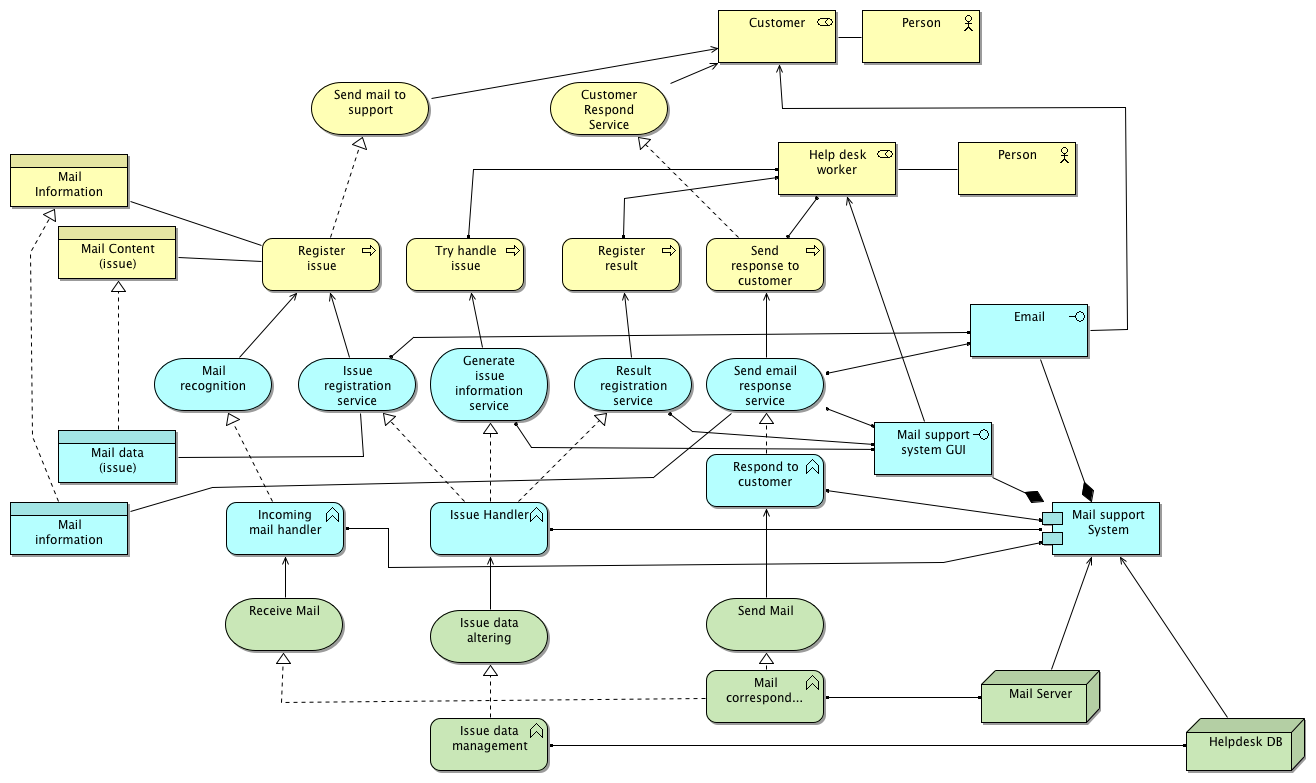
\includegraphics[scale = 0.25]{images/mailsupport.png}}
		\caption{Customer support via e-mail (\emph{ArchiMate})}
		\label{fig:archi_mail}
	\end{figure}
\end{center}
%

\subsection{MAP Analysis}
\label{sec:map_analysis}
This section contains analysis of segments of the As-Is MAP model, with respect to MAP attributes, where potential change could be made to reach the vision of the company.

\subsubsection{Order Registration - Cost}
\label{sec:order_analysis}
The registration of order application and sending the order acceptance letter as response are two processes which uses several systems and a role in the company. The role is an Order manager registering and sending acceptance letters. The systems he uses are order management systems, the order management database and the customer relation database. All this systems and the role seems quite costly for such a simple process, and to reach the vision of the company a more cost efficient architecture of these processes would help J.D.H. Insurance to provide better services and insurances. This architecture is interesting to analyze since it would be possible to replace the manager with an automated system and improve the usage of the order management system. The following view, \fref{fig:map_order_cost}, shows the view analyzed for finding cost in the processes which includes the manager.
\begin{center}
	\begin{figure}[H]
		\centering
		\setlength\fboxsep{7pt}
		\setlength\fboxrule{0.5pt}
		%\fbox{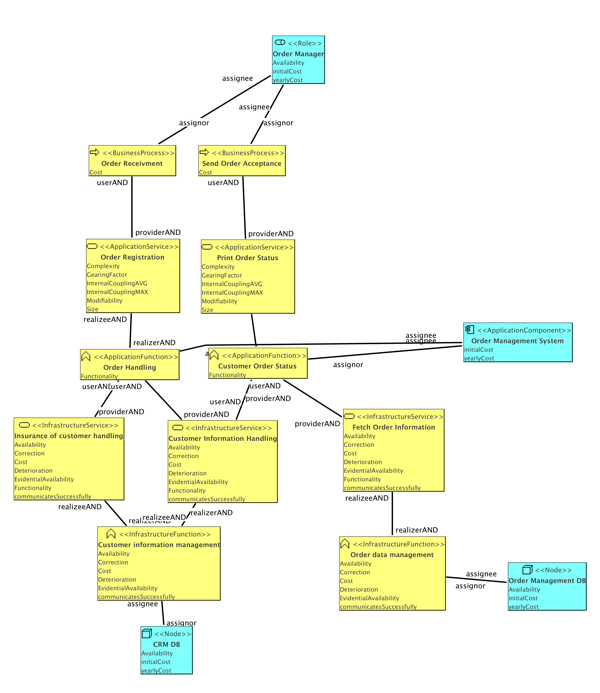
\includegraphics[scale = 0.35]{images/map_order_cost.png}}
		\caption{Cost of the processes "Order Receivement" and "Send Order Acceptance" (\emph{MAP})}
		\label{fig:map_order_cost}
	\end{figure}
\end{center}
The manager is a yearly cost for the company of 500' SEK, that includes salary and recruitment costs etc. The Order management system had an initial cost of 1500' SEK since its a large and complex system and a yearly cost of 300' SEK. The Order management database had an initial cost of 400' SEK and an yearly cost of 100' SEK. The CRM database is the most modern of these systems and was an initial cost of 700' SEK and is a yearly cost of 50' SEK.\\\\
%
The analysis resulted in a cost for the "Order receivement" process of 1525' SEK and a cost for the "Send Order Acceptance" process of 1837500 SEK.
%
\begin{table}[H]
	\centering
	\begin{tabular}{|c|c|p{2cm}|p{2.5cm}|p{2.5cm}|p{2.5cm}|}
		\cline{3-6}

		\multicolumn{2}{c}{} & \multicolumn{4}{|c|}{\textbf{Nodes}} \\ \cline{3-6}
		\multicolumn{2}{c|}{} & \multicolumn{2}{c|}{\textsl{CRM DB}} & \multicolumn{2}{c|}{\textsl{Order Management DB}} \\
		\hline
		\multicolumn{2}{|c|}{\textbf{Initial Cost}} & \multicolumn{2}{c|}{700 000} & \multicolumn{2}{c|}{400 000} \\ \hline
		\multicolumn{2}{|c|}{\textbf{Yearly Cost}}  & \multicolumn{2}{c|}{50 000} & \multicolumn{2}{c|}{100 000} \\ \hline
		
		\multicolumn{6}{c}{} \\ \cline{3-6}
		\multicolumn{2}{c}{} & \multicolumn{4}{|c|}{\textbf{Application Component}} \\ \cline{3-6}
		\multicolumn{2}{c|}{} & \multicolumn{4}{c|}{\textsl{Order Management System}} \\
		\hline
		\multicolumn{2}{|c|}{\textbf{Initial Cost}} & \multicolumn{4}{c|}{1 500 000}  \\ \hline
		\multicolumn{2}{|c|}{\textbf{Yearly Cost}}  & \multicolumn{4}{c|}{300 000}  \\ \hline

		
		\multicolumn{6}{c}{} \\ \cline{3-6}
		\multicolumn{2}{c}{} & \multicolumn{4}{|c|}{\textbf{Role}} \\ \cline{3-6}
		\multicolumn{2}{c|}{} & \multicolumn{4}{c|}{\textsl{Order Manager}} \\
		\hline
		\multicolumn{2}{|c|}{\textbf{Initial Cost}} & \multicolumn{4}{c|}{0}  \\ \hline
		\multicolumn{2}{|c|}{\textbf{Yearly Cost}}  & \multicolumn{4}{c|}{500 000}  \\ \hline


		\multicolumn{6}{c}{} \\ \cline{3-6}
		\multicolumn{2}{c}{} & \multicolumn{4}{|c|}{\textbf{Business Processes}} \\ \cline{3-6}
		\multicolumn{2}{c|}{} & \multicolumn{2}{c|}{\textsl{Order Receivement}} & \multicolumn{2}{c|}{\textsl{Send Order Acceptance}} \\
		\hline
		\multicolumn{2}{|c|}{\textbf{Cost}} & \multicolumn{2}{c|}{1 525 000} & \multicolumn{2}{c|}{1 875 000} \\ \hline

	\end{tabular}
\caption{Order process, \textsl{Cost} (As-Is)} 
\label{tab:order_cost_as_is}
\end{table}
%
\subsubsection{Order Registration - Service Availability}
\label{sec:order_availability}
In order to achieve maximum customer satisfaction the availability of the order registration service is crucial, as this currently is the sole entry point for customers intending to purchase an insurance. Consequently an increase in order availability could then help mitigate situations where a customer is unable to make an order due to system failure; and potentially missing out in a customer. In \fref{fig:map_order_availability}, the current as-is situation of order registration view is depicted.
\begin{center}
	\begin{figure}[H]
		\centering
		\setlength\fboxsep{7pt}
		\setlength\fboxrule{0.5pt}
		%\fbox{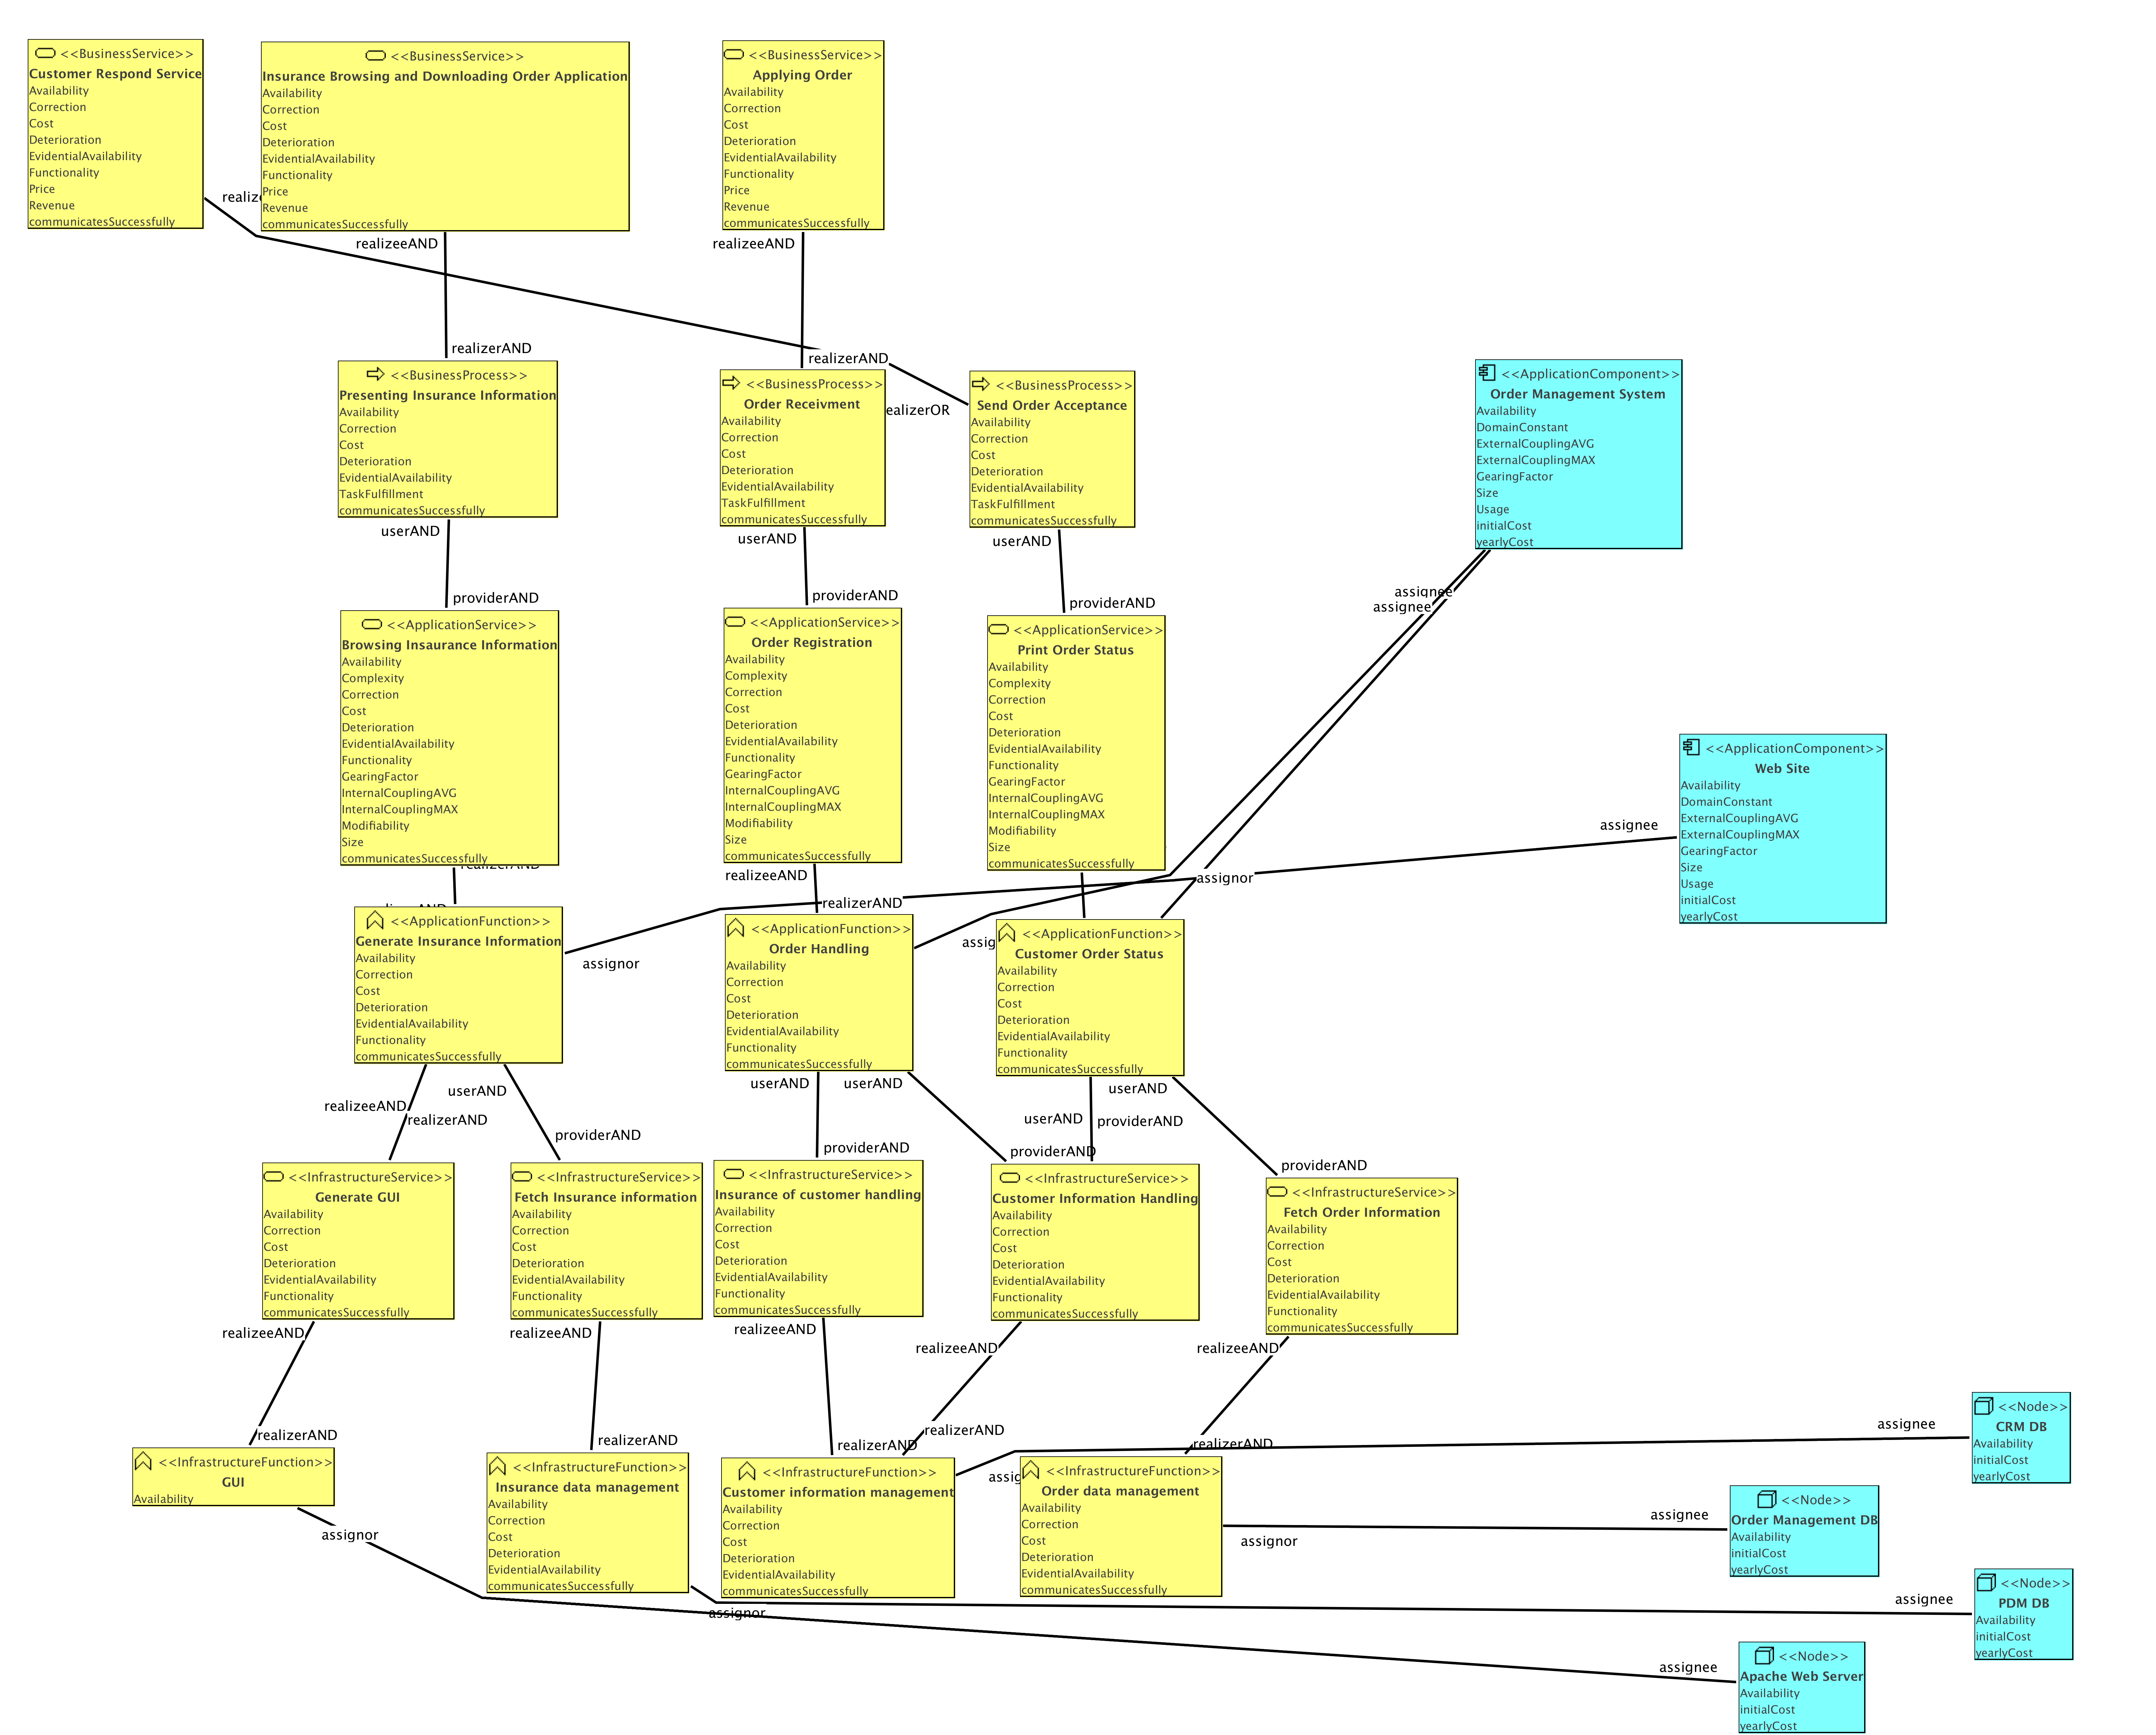
\includegraphics[scale = 0.05]{images/map_order_availability.png}}
		\caption{Cost of the processes "Order Receivement" and "Send Order Acceptance" (\emph{MAP})}
		\label{fig:map_order_availability}
	\end{figure}
\end{center}
Next we present the current values for some entities primarily considered when assessing the availability. The first two tables (Nodes \& Application components) are evidential values, meaning, that these are values already set and not computed with through the EAAT tool. Whereas the availability in table the last table are derived values by EAAT.
\begin{table}[H]
	\centering
	\begin{tabular}{|c|c|p{2cm}|p{2.5cm}|p{2.5cm}|p{2.5cm}|}
		\cline{3-6}

		\multicolumn{2}{c}{} & \multicolumn{4}{|c|}{\textbf{Nodes}} \\ \cline{3-6}
		\multicolumn{2}{c|}{}  & \multicolumn{2}{c|}{\textsl{CRM DB}} & \multicolumn{2}{c|}{\textsl{Order Management DB}} \\
		\hline
		\multicolumn{2}{|c|}{\textbf{Availability}} & \multicolumn{2}{c|}{0.99} & \multicolumn{2}{c|}{0.99} \\ \hline
		
		\multicolumn{6}{c}{} \\ \cline{3-6}
		\multicolumn{2}{c}{} & \multicolumn{4}{|c|}{\textbf{Application Component}} \\ \cline{3-6}
		\multicolumn{2}{c|}{} & \multicolumn{4}{c|}{\textsl{Order Management System}} \\
		\hline
		\multicolumn{2}{|c|}{\textbf{Availability}} & \multicolumn{4}{c|}{0.99} \\ \hline
		
		\multicolumn{6}{c}{} \\ \cline{3-6}
		\multicolumn{2}{c}{} & \multicolumn{4}{|c|}{\textbf{Role}} \\ \cline{3-6}
		\multicolumn{2}{c|}{} & \multicolumn{4}{c|}{\textsl{Order Manager}} \\
		\hline
		\multicolumn{2}{|c|}{\textbf{Availability}}  & \multicolumn{4}{c|}{0.95}  \\ \hline

		\multicolumn{6}{c}{} \\ \cline{3-6}
		\multicolumn{2}{c}{} & \multicolumn{4}{|c|}{\textbf{Business Processes}} \\ \cline{3-6}
		\multicolumn{2}{c|}{} & \multicolumn{2}{c|}{\textsl{Order Receivement}} & \multicolumn{2}{c|}{\textsl{Send Order Acceptance}} \\
		\hline
		\multicolumn{2}{|c|}{\textbf{Availability}} & \multicolumn{2}{c|}{0.92} & \multicolumn{2}{c|}{0.92} \\ \hline

		\multicolumn{6}{c}{} \\ \cline{3-6}
		\multicolumn{2}{c}{} & \multicolumn{4}{|c|}{\textbf{Business Services}} \\ \cline{3-6}
		\multicolumn{2}{c|}{} &  \multicolumn{4}{c|}{\textsl{Applying Order}}  \\
		\hline
		\multicolumn{2}{|c|}{\textbf{Availability}}  & \multicolumn{4}{c|}{0.92}\\ \hline

	\end{tabular}
\caption{Order process, \textsl{Service Availability} (As-Is)} 
\label{tab:order_as_is}
\end{table}

\subsubsection{Claim Registration - Data Accuracy}
\label{sec:claim_analysis}
The claim registration service which J.D.H. Insurance provide to the customers they insure has a critical point where it is important that the accuracy of the claims application maintain, that is when the claim administrator receives the claim application from an insurant and registers it into the claim management system. For J.D.H. Insurance to ensure that no information is lost in this process it is vital to analyze the data accuracy of it to see if it can be improved by a new architecture providing higher accuracy. The analyze is done by using the following view, displayed in figure 11.
\begin{center}
	\begin{figure}[H]
		\centering
		\setlength\fboxsep{7pt}
		\setlength\fboxrule{0.5pt}
		%\fbox{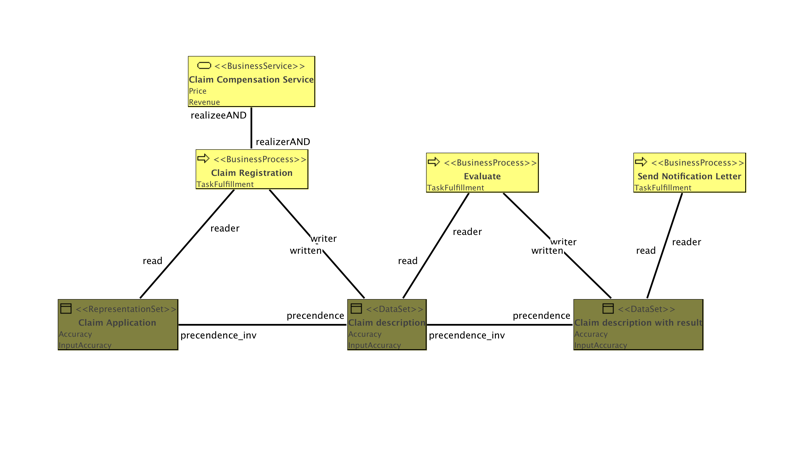
\includegraphics[scale = 0.35]{images/map_claim_data.png}}
		\caption{Data accuracy for the Claim data from received application to the evaluated claim object in the claim management system (\emph{MAP})}
		\label{fig:map_claim_data}
	\end{figure}
\end{center}
The claim application is sent by the insurant to the company and the input accuracy of the application can be assumed to be very high, 0.99. The application is processed by the claim administrator in the claim registration process and the translation from the paper application to the digital description tend to create loss of information, the deterioration of this process is 0.1. When the evaluator writes a result to the claim there is a small loss of information. The deterioration of this process is 0.03. \\\\ 
%
This results in a accuracy after the claim registration process of 0.89, and after the evaluation process an accuracy of 0.85, which seems like a low value for a company evaluating information provided by their customers and which aim to provide competitive insurances. Table x shows the values and the resulting accuracies in the process.
\begin{center}
\begin{table}[H]
\begin{tabular}{c|p{1.5cm}|p{1.5cm}|p{1.5cm}|p{1.5cm}|p{1.5cm}|p{1.7cm}|}

%\textbf{Attribute}& \textbf{State} & \textsl{Claim Application} & \textsl{Claim Description} & \textsl{Claim Description with result} & \textsl{Notification letter} \\

\cline{2-7}
	 & \multicolumn{6}{c|}{\textbf{Representation Sets (RS) and Data Sets (DS)}} \\ \cline{2-7}
	 & \textsl{Claim Application (RS)} & \textsl{Claim Description (RS)} & \textsl{Claim Description (DS)} & \textsl{Claim Description with Result (RS)} & \textsl{Claim Description with Result (DS)} & \textsl{Notification Letter (RS)}\\
\hline
\multicolumn{1}{|c|}{\textbf{Input Accuracy}} & 0.99 & 0.98 & 0.99 & 0.99 & 0.99 & 0.99\\ \hline
\multicolumn{1}{|c|}{\textbf{Accuracy}} & 0.99 & 0.89 & 0.88 & 0.85 & 0.85 & 0.84\\ \hline

	\multicolumn{7}{c}{} \\ \cline{2-7}
	& \multicolumn{6}{c|}{\textbf{Application Services}} \\ \cline{2-7}
	& \multicolumn{2}{c|}{\textsl{Register Claim Service}} & \textsl{Fetch Claim Description} & \textsl{Claim Result Service} & \multicolumn{2}{c|}{\textsl{Print Letter Service}} \\ \hline
	\multicolumn{1}{|c|}{\textbf{Deterioration}} & \multicolumn{2}{c|}{0.01} & 0.01 & 0.01 & \multicolumn{2}{c|}{0.01} \\ \hline

	\multicolumn{7}{c}{} \\ \cline{2-7}
	& \multicolumn{6}{c|}{\textbf{Business Processes}} \\ \cline{2-7}
	& \multicolumn{3}{c|}{\textsl{Claim Registration}} & \multicolumn{3}{c|}{\textsl{Evaluate}} \\ \hline
	\multicolumn{1}{|c|}{\textbf{Deterioration}} & \multicolumn{3}{c|}{0.10} & \multicolumn{3}{c|}{0.03} \\ \hline
%\multicolumn{2}{c}{} & \multicolumn{4}{|c|}{\textbf{Business process}} \\ \cline{3-6}
%\multicolumn{2}{c|}{} & \multicolumn{4}{|c|}{\textsl{Claim Registration}} \\ \hline
%\multicolumn{2}{|c|}{\textbf{Deterioration}} & \multicolumn{4}{|c|}{0.15}\\ \hline
\end{tabular}
\caption{Claim process, \textsl{Data Accuracy} (As-Is)}
\label{tab:claim_as_is}
\end{table}
\end{center}
%
\subsubsection{Support - Service Availability}
\label{sec:support_analysis}
One of J.D.H. Insurance visions is to provide the good support for their customers. One important aspect of this support is the availability of the support. Clearly the access points for the support functions need to be available to the customers if they should be able to contact J.D.H. Insurance. An analysis of the availability of the access points of both the support architectures would then be of value for J.D.H. Insurance, and to evaluate what improvements that could be done to increase the availability of these services. The following view, figure 12, shows the service of calling to the phone support and analyzes its availability to the customers, and figure x displays the access point of mail support analyzed.
\begin{center}
	\begin{figure}[H]
		\centering
		\setlength\fboxsep{7pt}
		\setlength\fboxrule{0.5pt}
		%\fbox{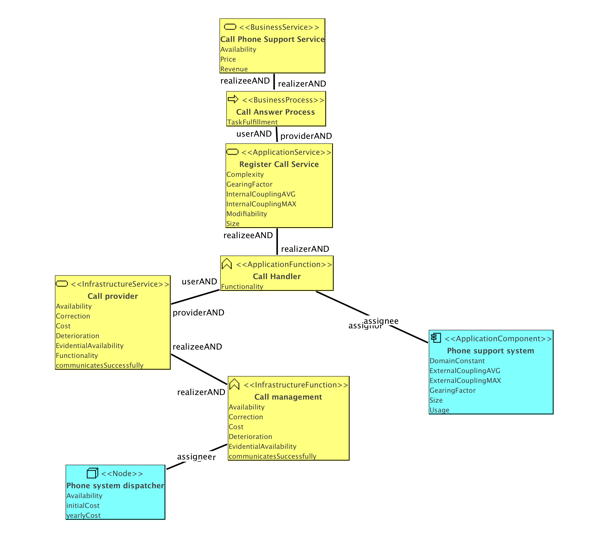
\includegraphics[scale = 0.35]{images/map_support_phone_availability.png}}
		\caption{Service availability of the Phone support access service (\emph{MAP})}
		\label{fig:map_support_phone_availability}
	\end{figure}
\end{center}
Table x contains the values for each availability of the systems in the phone support process. The result of the analysis of these values gives an availability of 0.85 for the Contact phone support service, which is a low value for a service which should be able to compete with other companies similar services.
\begin{center}
	\begin{figure}[H]
		\centering
		\setlength\fboxsep{7pt}
		\setlength\fboxrule{0.5pt}
		%\fbox{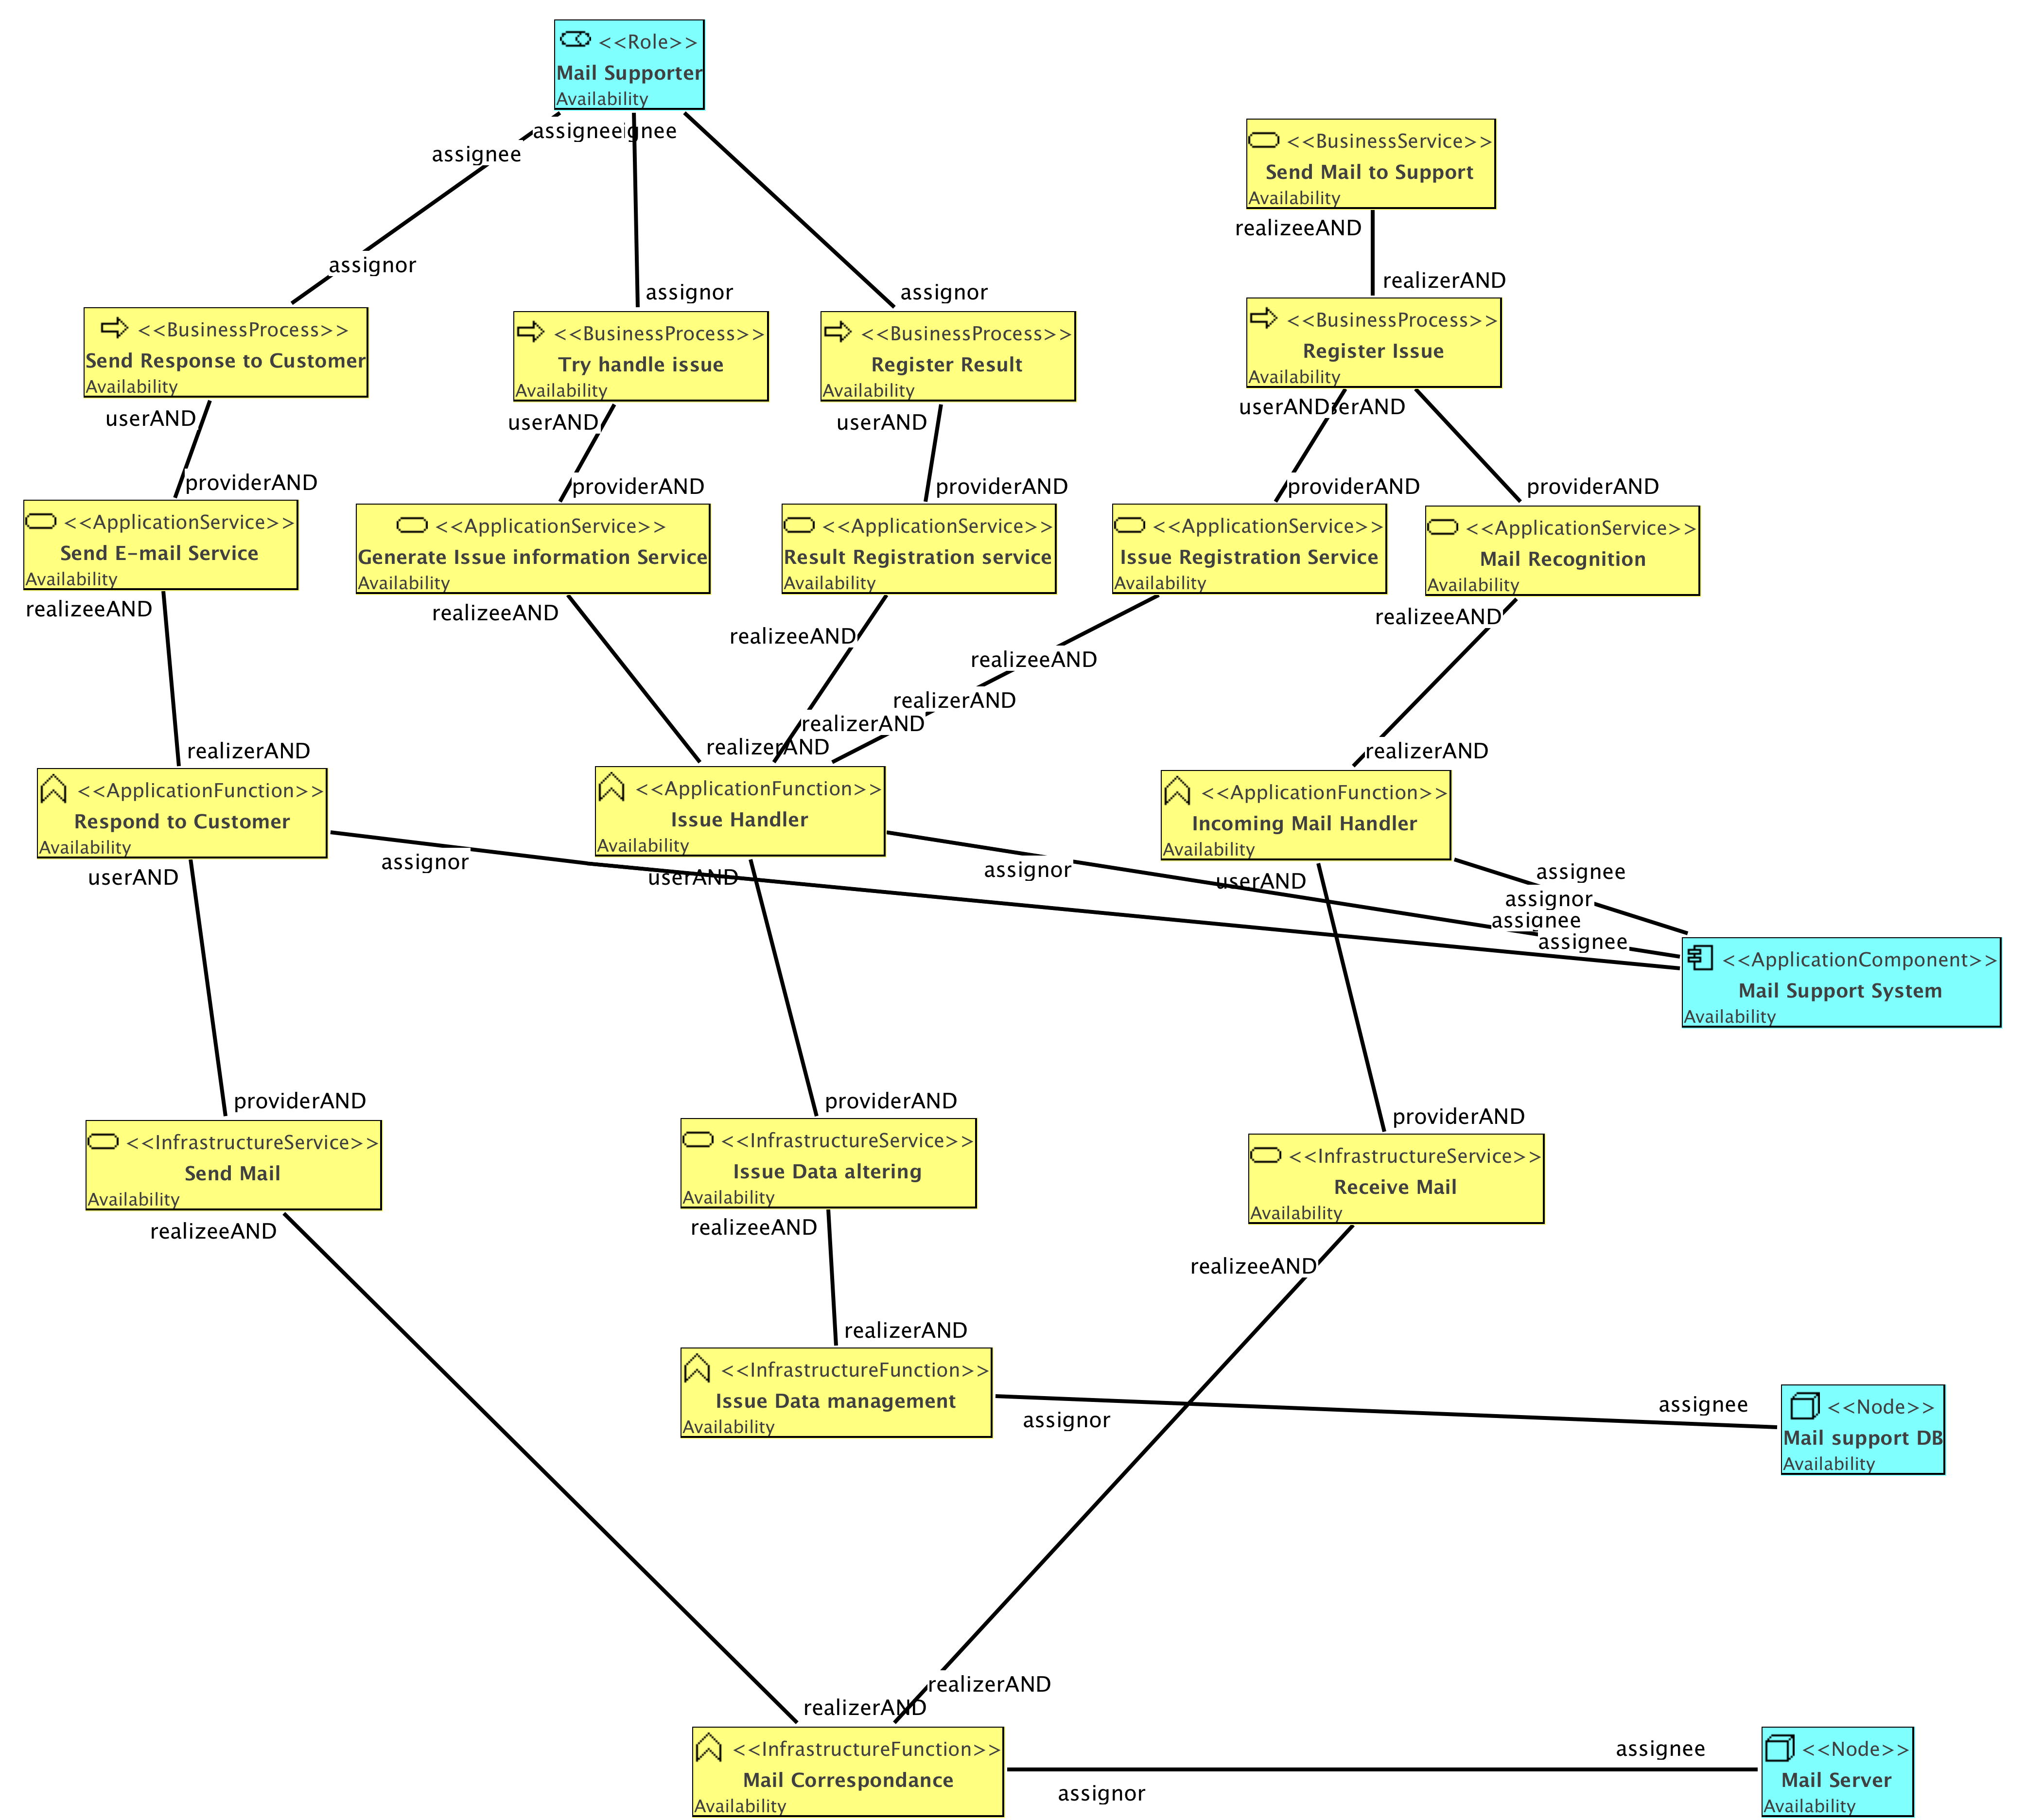
\includegraphics[scale = 0.09]{images/map_support_email_availability.png}}
		\caption{Service availability of the Mail support service (\emph{MAP})}
		\label{fig:map_support_mail_availability}
	\end{figure}
\end{center}

\begin{table}[H]
	\centering
	\begin{tabular}{|c|c|p{2.5cm}|p{2.5cm}|p{2.5cm}|p{2.5cm}|}

		%\multicolumn{2}{c}{} & \multicolumn{1}{p{2.5cm}}{} & \multicolumn{2}{p{5cm}}{} & \multicolumn{1}{p{2.5cm}}{} \\ %ALLIGNER!
		\cline{3-6}

		\multicolumn{2}{c}{} & \multicolumn{4}{|c|}{\textbf{Nodes}} \\ \cline{3-6}
		\multicolumn{2}{c|}{} & \multicolumn{1}{|c|}{\textsl{Phone System Dispatcher}} & \multicolumn{1}{|c|}{\textsl{Phone Support DB}} & \multicolumn{1}{|c|}{\textsl{Mail Server}} &\multicolumn{1}{|c|}{\textsl{Mail DB}} \\ \hline
		\multicolumn{2}{|c|}{\textbf{Availability}} & \multicolumn{1}{|c|}{0.97} & \multicolumn{1}{|c|}{0.97} & \multicolumn{1}{|c|}{0.98} & \multicolumn{1}{|c|}{0.96} \\  \hline

		\multicolumn{6}{c}{} \\ \cline{3-6}							
		\multicolumn{2}{c}{} & \multicolumn{4}{|c|}{\textbf{Application Components}} \\ \cline{3-6}
		\multicolumn{2}{c|}{} & \multicolumn{2}{c|}{\textsl{Phone Support System}} & \multicolumn{2}{c|}{\textsl{Mail Support System}} \\
		\hline
		\multicolumn{2}{|c|}{\textbf{Availability}} & \multicolumn{2}{c|}{0.98} & \multicolumn{2}{c|}{0.98} \\ \hline

	   \multicolumn{6}{c}{} \\ \cline{3-6}
		\multicolumn{2}{c}{} & \multicolumn{4}{|c|}{\textbf{Role}} \\ \cline{3-6}
		\multicolumn{2}{c|}{} & \multicolumn{2}{|c|}{\textsl{Phone Supporter}} & \multicolumn{2}{|c|}{\textsl{Mail Supporter}}\\ \hline
		\multicolumn{2}{|c|}{\textbf{Availability}}& \multicolumn{2}{|c|}{0.97} & \multicolumn{2}{|c|}{0.95}\\  \hline
		
		\multicolumn{6}{c}{} \\ \cline{3-6}
		\multicolumn{2}{c}{} & \multicolumn{4}{|c|}{\textbf{Business Services}} \\ \cline{3-6}
		\multicolumn{2}{c|}{} & \multicolumn{1}{|c|}{\textsl{Contact Phone Support}} & \multicolumn{2}{|c|}{\textsl{Contact Email Support}} & \multicolumn{1}{|p{2cm}|}{\textsl{Respond to Customer}}\\ \hline
		\multicolumn{2}{|c|}{\textbf{Availability}}& \multicolumn{1}{|c|}{0.85} & \multicolumn{2}{|c|}{0.90} & \multicolumn{1}{|c|}{0.91}\\ \hline
	\end{tabular}
\caption{Support process, \textsl{Service Availability} (As-Is)} 
\label{tab:support_as_is}
\end{table}
Table x displays the availabilities of the systems in the mail support process. The analysis results in an availability of the Contact mail support service of 0.90, which seems quite low for both being a mail service and for being an important service to customers.\\\\
%
\emph{Note: We experienced problems with EAAT during this analysis. EAAT did not calculate a distinct value for the Register issue process. The availability has been calculated manually, using multiplication of the two availabilities of the application services Issue Registration Service and Mail Recognition.}
%
\subsection{Improvements}
\label{sec:improvements}
J.D.H Insurance could apply many changes to their main processes to align with the goals of this report. This section presents improvements for certain attributes in the MAP metamodel to certain processes and services.
\subsubsection{Order Process (Cost/Availability)}
The order process uses many different systems for fulfilling its purpose, along with an employee working for registering these orders and sending letter back to the customers about their order. These systems and the employees are quite costly and as the process is very important to J.D.H Insurance and a process which will remain in the company a reduction of these costs are motivated.
\subsubsection{Claim Process (Accuracy)}
As the claim process suffers of low accuracy in the processing of a claim application, a clear improvement for reaching the vision of being a leading company is to increase the accuracy of this process. As mentioned in the goals of this report, it would support the decision making of compensating the customer for her claim or not, which has an interest for both J.D.H. Insurance and their customers.
\subsubsection{Support Services (Availability)}
The support services are important services for the customers and its availability is an important factor in the customers satisfaction of being a customer in J.D.H Insurance. An increase of the availability of the mail support and the phone support would increase the customers satisfaction which in turn could impact the new customer stream to the company and thereby revenue.